\documentclass[letterpaper]{article}

\usepackage[left=0.8in,top=0.8in,right=0.8in,bottom=0.8in]{geometry} % margins

\usepackage{lmodern}
\usepackage[T1]{fontenc}
\usepackage{pxfonts}

\usepackage{graphics}
\usepackage{tikz}
\usetikzlibrary{shadows,arrows,shapes,decorations.pathmorphing,backgrounds,positioning,fit,petri,matrix,graphs}
\usetikzlibrary{calc}

\definecolor{darkgray}{rgb}{0.4,0.4,0.4}
\definecolor{gblue1}{rgb}{1.0,0.6,0.6}
\definecolor{blue2}{rgb}{0.5,0.7,1.0}
\definecolor{lightgreen}{rgb}{0.9,1.0,0.9}
\definecolor{lightblue}{rgb}{0.9,0.9,1.0}
\definecolor{turquoise}{rgb}{0.3,0.9,0.8}
\definecolor{aquamarine}{rgb}{0.5,1.0,0.8}
\definecolor{orchid}{rgb}{0.8,0.6,0.7}
\definecolor{darkorangered}{rgb}{0.95,0.3,0.1}
\definecolor{darkred}{rgb}{0.95,0.0,0.0}
\definecolor{orange}{rgb}{0.9,0.6,0.3}

\tikzset{
  basic/.style  = {draw, text width=2cm, drop shadow, rectangle},
  root/.style   = {basic, rounded corners=2pt, thin, align=center, fill=green!30},
  box-round-1/.style = {basic, rounded corners=4pt, thin, align=center, fill=lightblue, text width=12em, text height=1em},
  box-round-2/.style = {basic, rounded corners=4pt, thin, align=center, fill=lightgreen, text width=12em, text height=1em},
  box-round-3/.style = {basic, rounded corners=4pt, thin, align=center, fill=turquoise!40, text width=9em, text height=0.8em},
  box-round-4/.style = {basic, rounded corners=4pt, thin, align=center, fill=blue!16, minimum size=2.2cm},
  bend angle=45,
  in-arrow/.style={<-,shorten <=1pt,>=stealth',thick},
  out-arrow/.style={->,shorten >=1pt,>=stealth',thick}
}

\pgfdeclareimage[interpolate=true,width=1.2cm,height=1.2cm]{image-electrum}{/home/tarok/Finance/Bitcoin/Electrum/electrum.png}

\begin{document}

\pagestyle{empty}

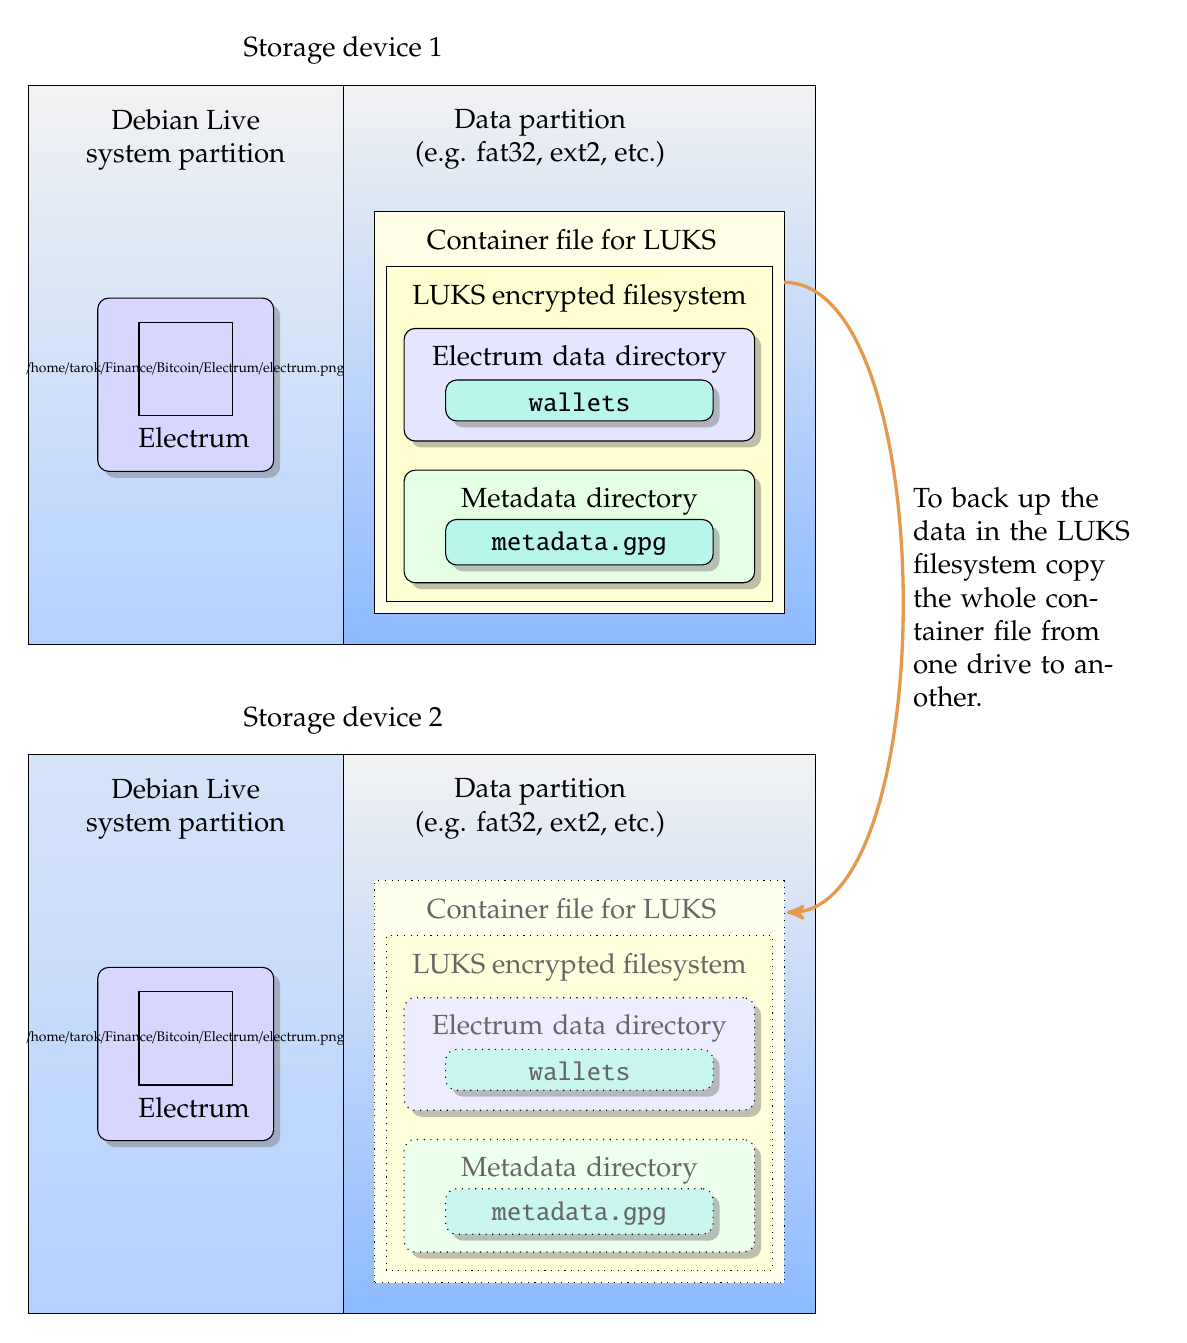
\begin{tikzpicture}

  \draw[top color=gray!10!, bottom color=blue2!60!] (0.0,8.5) rectangle (4.0,15.6);
  \draw[top color=gray!10!, bottom color=blue2!90!] (4.0,8.5) rectangle (10.0,15.6);

  \draw (4.0,15.6) node[above=4pt,align=center] (storage-1) {Storage device 1};
  \draw (2.0,15.6) node[below=5pt,align=center] {Debian Live\\ system partition};
  \draw (6.5,15.6) node[below=5pt,align=center] {Data partition\\ (e.g. fat32, ext2, etc.)};

  \draw[top color=yellow!09!, bottom color=yellow!09!]  (4.4,8.9) rectangle (9.6,14.0);
  \draw[top color=yellow!18!, bottom color=yellow!18!]  (4.55,9.05) rectangle (9.45,13.3);
  \draw (6.9,14.0) node[below=3pt,align=center] (container-1) {Container file for LUKS};
  \draw (7.0,13.3) node[below=3pt,align=center] (luks-title-1) {LUKS encrypted filesystem};

  \draw (7.0,11.8) node[box-round-1,align=center] (data-dir-1) {Electrum data directory\\ \hspace{1em}\\ \hspace{1em}};
  \draw (7.0,11.6) node[box-round-3,align=center] (wallets-1) {\texttt{wallets}};
  \draw (7.0,10.0) node[box-round-2,align=center] (metadata-dir-1) {Metadata directory\\ \hspace{1em}\\ \hspace{1em}};
  \draw (7.0,9.8) node[box-round-3,align=center] (metadata-1) {\texttt{metadata.gpg}};

  \draw (2.0,11.8) node[box-round-4,align=center] (icon-box-1) {};
  \pgftext[at=\pgfpoint{1.4cm}{11.4cm},left,base]{\pgfuseimage{image-electrum}}
  \pgftext[at=\pgfpoint{1.4cm}{11.0cm},left,base]{Electrum}


  \draw[top color=gray!10!, bottom color=blue2!60!] (0.0,0.0) rectangle (4.0,7.1);
  \draw[top color=gray!10!, bottom color=blue2!90!] (4.0,0.0) rectangle (10.0,7.1);

  \draw (4.0,7.1) node[above=4pt,align=center] (storage-2) {Storage device 2};
  \draw (2.0,7.1) node[below=5pt,align=center] {Debian Live\\ system partition};
  \draw (6.5,7.1) node[below=5pt,align=center] {Data partition\\ (e.g. fat32, ext2, etc.)};

  \draw[top color=yellow!07!, bottom color=yellow!07!,dotted]  (4.4,0.4) rectangle (9.6,5.5);
  \draw[top color=yellow!14!, bottom color=yellow!14!,dotted]  (4.55,0.55) rectangle (9.45,4.8);
  \draw (6.9,5.5) node[below=3pt,align=center,dotted] (container-2) {\textcolor{darkgray}{Container file for LUKS}};
  \draw (7.0,4.8) node[below=3pt,align=center] (luks-title-2) {\textcolor{darkgray}{LUKS encrypted filesystem}};

  \draw (7.0,3.3) node[box-round-1,align=center,dotted,fill=lightblue!70!] (data-dir-2) {\textcolor{darkgray}{Electrum data directory\\ \hspace{1em}\\ \hspace{1em}}};
  \draw (7.0,3.1) node[box-round-3,align=center,dotted,fill=turquoise!30!] (wallets-2) {\textcolor{darkgray}{\texttt{wallets}}};
  \draw (7.0,1.5) node[box-round-2,align=center,dotted,fill=lightgreen!70!] (metadata-dir-2) {\textcolor{darkgray}{Metadata directory\\ \hspace{1em}\\ \hspace{1em}}};
  \draw (7.0,1.3) node[box-round-3,align=center,dotted,fill=turquoise!30!] (metadata-2) {\textcolor{darkgray}{\texttt{metadata.gpg}}};

  \draw (2.0,3.3) node[box-round-4,align=center] (icon-box-2) {};
  \pgftext[at=\pgfpoint{1.4cm}{2.9cm},left,base]{\pgfuseimage{image-electrum}}
  \pgftext[at=\pgfpoint{1.4cm}{2.5cm},left,base]{Electrum}

  \draw[out-arrow,very thick,orange] (9.6,13.1) .. controls +(0:2cm) and +(0:2cm) .. (9.6,5.1) node[midway,right,text width=3cm]
       {\textcolor{black}{To back up the data in the LUKS filesystem copy the whole container file from one drive to another.}};

\end{tikzpicture}

\end{document}
